\documentclass[letterpaper,12pt]{article}

%%%%%%%%%%%%%%%%%%%%%%% PDF Output %%%%%%%%%%%%%%%%%%%%%%%%%%%%%%%%%%%%
\newif\ifpdf
\ifx\pdfoutput\undefined
  \pdffalse     % not running PDFLaTeX
\else
  \pdfoutput=1  % running PDFLaTeX
  \pdftrue
\fi
\ifpdf
  \usepackage[pdftex]{graphicx}
  \usepackage[pdftex]{hyperref} 
  \DeclareGraphicsExtensions{.jpg,.pdf,.png,.mps}
\else
  \usepackage[dvips]{graphicx}
  \usepackage[dvips]{hyperref} 
\fi

%%%%%%%%%%%%%%%%%%%%%%%% Standard Packages %%%%%%%%%%%%%%%%%%%%%%%%%%%%
\usepackage{epsfig}
\usepackage{amssymb}
\usepackage{amsmath}
\usepackage{mathrsfs}
\usepackage{fancyvrb}
\usepackage{caption}
\usepackage{comment}
\usepackage{fancyhdr}
\usepackage{subfigure}
\usepackage{clrscode}

%%%%%%%%%%%%%%%%%%%%%%%% Adapted from Sweave %%%%%%%%%%%%%%%%%%%%%%%%%%
\DefineVerbatimEnvironment{Rcode}{Verbatim}{fontshape=sl, frame=single, 
  framesep=2mm, fontsize=\small, baselinestretch=.5}

%%%%%%%%%%%%%%%%%%%%%%%%%%%%%%%%%%%%%%%%%%%%%%%%%%%%%%%%%%%%%%%%%%%%%%%

%%%%%%%%% My macros (which of course are borrowed from a million ... %%
\def\argmax{\operatornamewithlimits{arg\,max}}
\def\argmin{\operatornamewithlimits{arg\,min}}


%%%%%%%%%%%%%%%%%%%%%%%% Page and Document Setup %%%%%%%%%%%%%%%%%%%%%%%
\addtolength{\oddsidemargin}{-0.875in}
\addtolength{\topmargin}{-0.875in}
\addtolength{\textwidth}{1.75in}
\addtolength{\textheight}{1.75in}

\captionsetup{margin=15pt,font=small,labelfont=bf}

\renewcommand{\topfraction}{0.9}        % max fraction of floats at top
\renewcommand{\bottomfraction}{0.8}     % max fraction of floats at bottom

% Parameters for TEXT pages (not float pages):
\setcounter{topnumber}{2}
\setcounter{bottomnumber}{2}
\setcounter{totalnumber}{4}             % 2 may work better
\setcounter{dbltopnumber}{2}            % for 2-column pages
\renewcommand{\dbltopfraction}{0.9}     % fit big float above 2-col. text
\renewcommand{\textfraction}{0.07}      % allow minimal text w. figs

% Parameters for FLOAT pages (not text pages):
\renewcommand{\floatpagefraction}{0.7}          % require fuller float pages

% N.B.: floatpagefraction MUST be less than topfraction !!
\renewcommand{\dblfloatpagefraction}{0.7}       % require fuller float pages


%%%%%%%%%%%%%%%%%%%%%%% options for sweave %%%%%%%%%%%%%%%%%%%%%%%%%%%%%
% \SweaveOpts{prefix.string=plots/lab4}

%%%%%%%%%%%%%%%%%%%%%% headers and footers %%%%%%%%%%%%%%%%%%%%%%%%%%%%%
\pagestyle{fancy} 
\renewcommand{\footrulewidth}{\headrulewidth}

%%%%%%%%%%%%%%%%%%%%%%%%% bibliography  %%%%%%%%%%%%%%%%%%%%%%%%%%%%%%%%
% \bibliographystyle{plainnat}
\bibliographystyle{plain}

%%%%%%%%%%%%%%%%%%%%%%%%%%%%%%%%%%%%%%%%%%%%%%%%%%%%%%%%%%%%%%%%%%%%%%%%
%%%%%%%%%%%%%%%%%%%%%%%%% Now Edit %%%%%%%%%%%%%%%%%%%%%%%%%%%%%%%%%%%%%
%%%%%%%%%%%%%%%%%%%%%%%%%%%%%%%%%%%%%%%%%%%%%%%%%%%%%%%%%%%%%%%%%%%%%%%%
\fancyhead[L]{\em panjo}
\fancyhead[R]{\em CS 267}
\fancyfoot[L]{\em \today}
\fancyfoot[C]{}
\fancyfoot[R]{\em \thepage}


%%%%%%%%%%%%%%%%%%%%%%% opening %%%%%%%%%%%%%%%%%%%%%%%%%%%%%%%%%%%%%%%%
\title{panjo: a parallel neighbor joining algorithm}
\author{James Bullard}
\begin{document}
\maketitle
\tableofcontents
%% \listoffigures

\section{Introduction}
In this report we present a parallel implementation of the popular
neighbor joining algorithm used frequently to reconstruct phylogenetic
trees. The neighbor joining algorithm was initially proposed by
Saitou, N. and Nei, M. \cite{saitou1987the} and then revised by
J.A. Studier, K.J. Keppler \cite{studier_kepler_1988}. In this report
we will investigate the revised algorithm which has been shown to be
an order $O(n^3)$ algorithm. The structure of the report is as
follows:

Briefly, phylogentic trees are used to represent the relationships
between evolving species. Classically, we think of the phylogenetic
tree of the higher primates or the phylogentic tree depicted in figure
(\ref{fig:ex_tree}). Trees can be constructed using visibibly
observable features, expressed proteins, or in many cases
genetic sequences. In this report, we use the language of
genetic sequences when we describe things, however it should be
noted that if suitably defined other discriminatory features can be
used with the same methods. There has been an explosion of data in the
last 10 years and this explosion of data has allowed us to examine
phylogenies of larger and larger sizes. The software developed for
this report was designed with this in mind. Often, in bioinformatics,
we have such large data sets that is a challenge to compute on
them. The ``panjo'' software package has been designed with this
constraint in mind. In the particular database our collaborators
maintain \cite{desantis_greengenes} there are over 140,000
sequences which have been found in the environment. We wish to
construct a phylogenetic tree for this massive data set, but no
currently available tools allows for such construction.  

\subsection{Building Phylogenetic Trees}
Many methods have been proposed to build phylogentic trees. Broadly
these methods can be viewed as coming from either two classes -
Maximum Likelihood based methods or Distance based methods. The
maximum liklihood based methods often suffer from an exponential time
scaling problem so their usage on large trees is generally
impossible. Current best guesses as to the number of sequences which
one could possibly hope to assemble using maximum likelihood methods
into a phylogenetic tree are on the order of tens of thousands.

The second class of methods do not suffer from such poor
scaling. These methods utilize a distance matrix to define pairwise
distances between any two sequences. This distance matrix becomes the
focal point of the computation. These algorithms have their own
problems as we shall see. Firstly, they generally have least $O(N^2)$
space requirements. The most popular algorithm neighbor-joining is
$O(N^3)$ in time complexity and $O(N^2)$ in space complexity. There
have naturally been improvements to these constraints, but generally
at the cost of relaxation of the algorithms intents. The main problem
which we will see with the effective parallelization of the algorithm
comes down to load-balancing issues as well as a good deal of 

\subsubsection{Current Limitation}

\subsection{The Neighbor-Joining Algorithm}

\section{Methods}
\subsection{Assessing Performance}
Now that we have a better understanding of the algorithm which we wish
to parallelize we can better understand how good we can expect to
do. Furthermore, we can then propose a performance model 

\subsection{Parallel Implementation}
\begin{figure}
\centering 
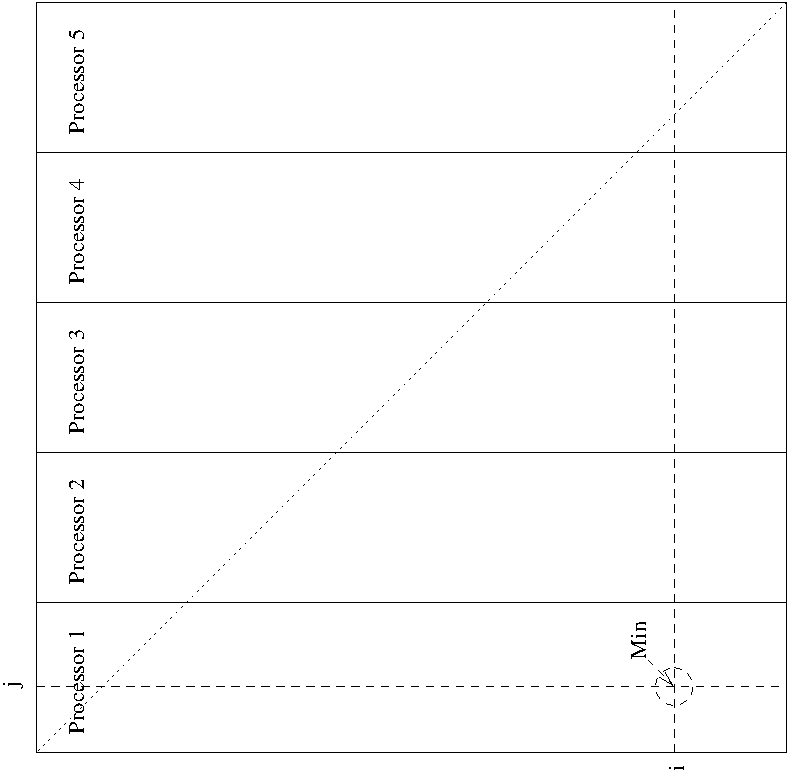
\includegraphics[angle=-90]{fig_mat.pdf}
\caption{Step 1: The matrix at the beginning of the computation. Each process
  computes its minimum reweighted value. The processors exchange and a
  global minimum value (Min) is found.}
\label{fig:mat_1}
\end{figure}

\begin{figure}
\centering 
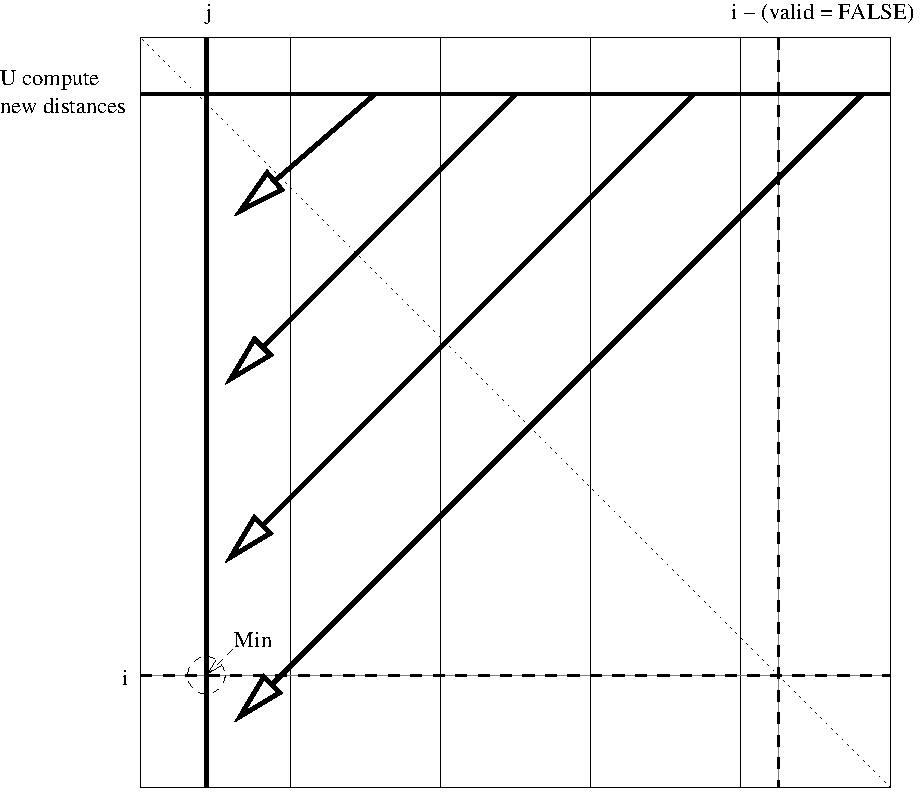
\includegraphics[]{fig_mat3.pdf}
\caption{Step 2: The row and column corresponding to i are eliminated
  from future work. The new node U is added and distances to it and
  every other node are computed. Each processor computes its
  corresponding piece and then the pieces are sent to the processor
  which owns column J; This is effectively a row-column transpose operation.}
\label{fig:mat_2}
\end{figure}

\begin{codebox} 
  \Procname{$\proc{ProduceOrdering}(G, JT)$} 
  \zi \Comment we operate on the cliques - therefore our methods such
  \zi \Comment as getParent, remove, getChildren, etc. operate on
  \zi \Comment cliques. 
  \zi
  \zi \id{ordering} = \{\}
  \zi \proc{Descend}(\func{getRoot}(JT))
  \zi \func{return}(\func{reverse}(\id{ordering})
  \zi
  \zi \proc{Descend}($clique$)
  \zi \> \If (\func{hasChildren}($clique$))
  \zi \Then
  \zi \For $\nu_i \in$ \func{getChildren}($clique$)
  \zi \Do
  \zi \> \proc{Descend}($\nu_i$)
  \zi \End
  \zi \Else
  \zi \Comment $D$ are nodes of the graph.
  \zi \> D = $clique$ - \func{getParent}($clique$)
  \zi \> \func{push}(D, ordering)
  \zi \> \func{remove}($clique$)
  \zi \End
  \zi \End
\end{codebox} 




\section{Results}
\subsection{Overall Performance}
We present performance plots for the following case. Distance matrices
of sizes $(1000, 2000, 3000, 4000, 5000, 6000, 7000, 8000, 10000)$ were
used on the following numbers of processors: $(1, 2, 4, 5, 10, 20,
40)$. In figure (\ref{fig:performance}) we show the wall time for each
matrix with a separate line representing the number of processors
used. We note that for some larger matrix sizes and smaller processor
numbers all matrix sizes were not computed. We did however compute all
matrix sizes for 1 processor to accurately report speedup and parallel
efficiency.
\begin{figure}[!ht]
  \centering 
  \subfigure[Total run time for each matrix size and processor combination]{%
    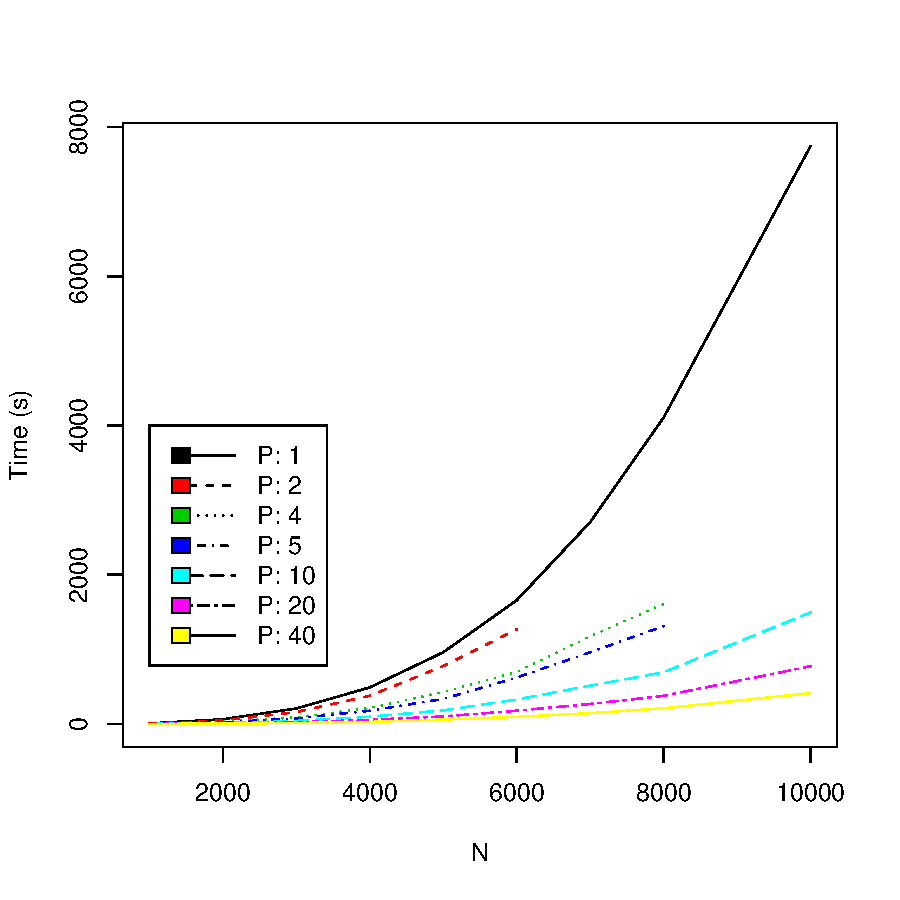
\includegraphics[width = 0.45\textwidth]{plots/performance.pdf}}
  \hspace{0.3in}%
  \subfigure[Time spent in MPI routines divided by Total run time.]{%
    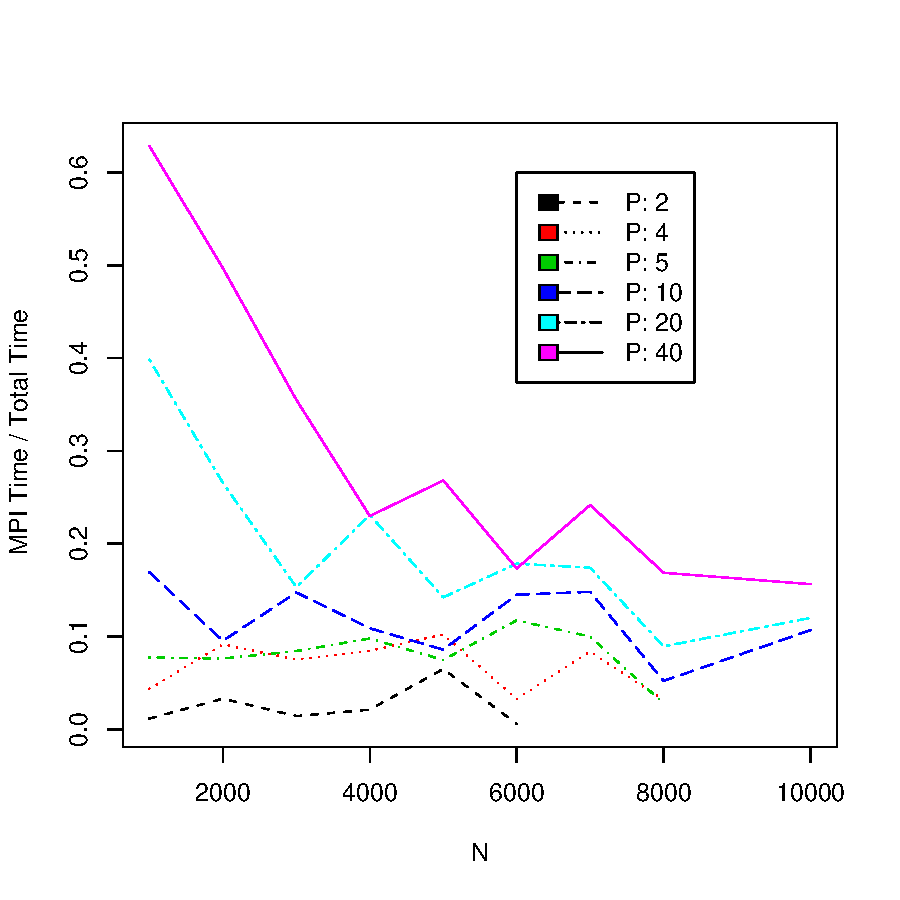
\includegraphics[width = 0.45\textwidth]{plots/mpi_performance.pdf}}
  \caption{Performance of both serial implementation both with respect
    to total time as well as the ratio of time spent in MPI to the total
    time.}
  \label{fig:performance}
\end{figure}

\subsection{Parallel Efficiency/Speedup}
In figure (\ref{fig:speedup}) we now present parallel efficiency and speedup plots. We recall that
under the observations that there is a smaller amount of parallelism
which we might hope to eek out of the algorithm while ensuring
correctness to the serial version we are quite pleased with the
speedup plots. In terms of the parallel efficiency plots we note that
it would be much more helpful to have much larger matrices to gauge
how the things behave for extremely large distance matrices. We also
need to declare that our single processor implementation was not
optimized. However, it is comparable to other packages in terms of
absolute performance. One nice implementation aspect is that the
serial and parallel versions can be conditionally compiled.
\begin{figure}[!ht]
  \centering 
  \subfigure[Speedup]{%
    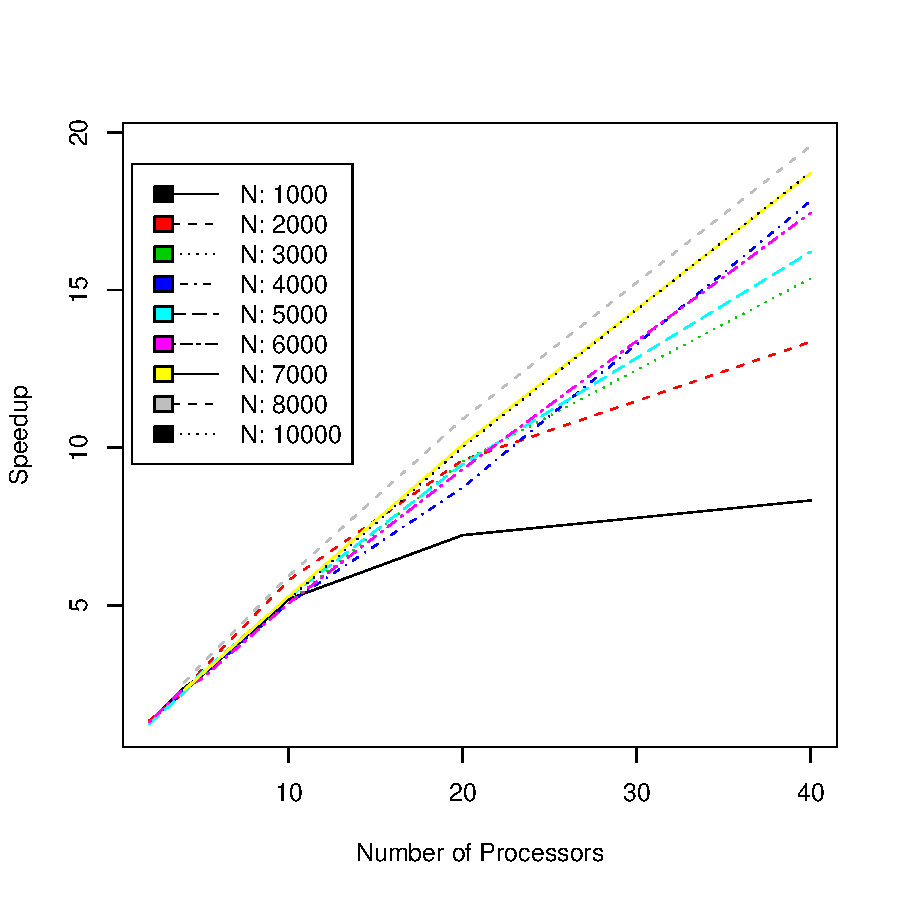
\includegraphics[width = 0.45\textwidth]{plots/speedup.pdf}}
  \hspace{0.3in}%
  \subfigure[Parallel efficiciency]{%
    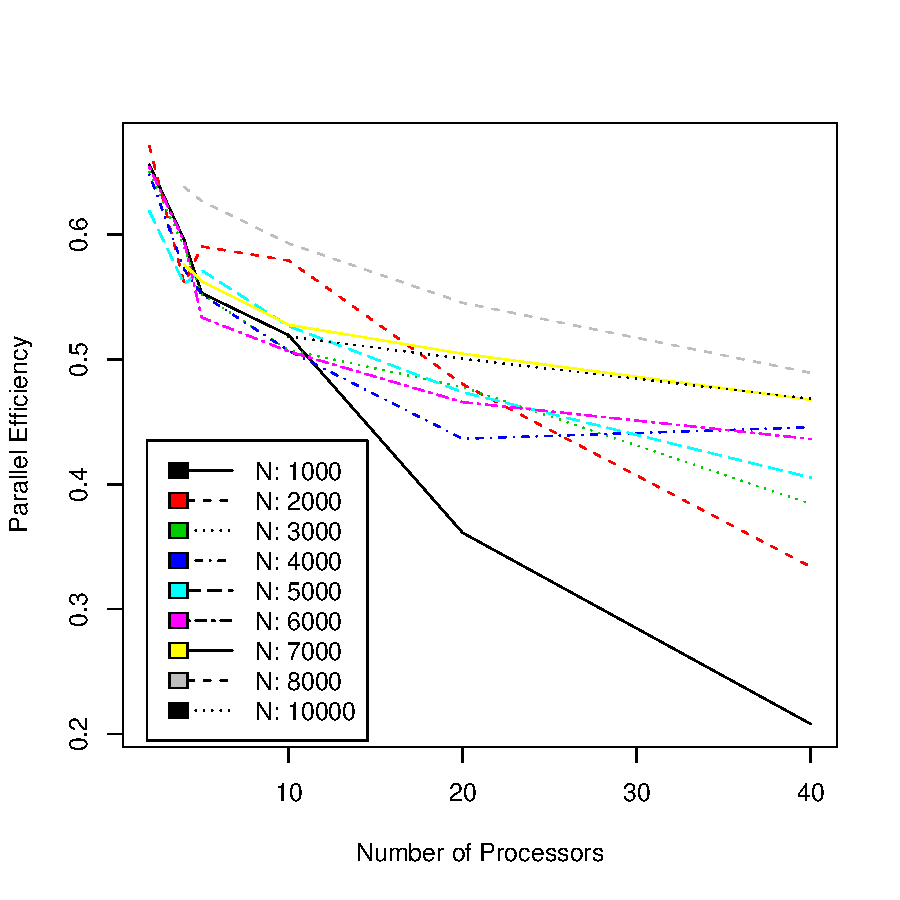
\includegraphics[width = 0.45\textwidth]{plots/efficiency.pdf}}
  \caption{Speedup and Efficiency plots}
  \label{fig:speedup}
\end{figure}


\section{Conclusions}

\bibliography{panjo.bib}
\end{document}

